\documentclass{article}
\usepackage[T1]{fontenc}
\usepackage{imakeidx}
\usepackage{graphicx} %package to manage images
\graphicspath{ {./images/} }
\usepackage[rightcaption]{sidecap}
\usepackage{wrapfig}
\makeindex[columns=3, title=Alphabetical Index, intoc]

\clearpage

\begin{document}


\begin{titlepage}
    \begin{center}
            
        \Large
            
        Practical work report
        \\ Language Processing
            
        \vspace{0.8cm}
            
        
\includegraphics[width=0.8\textwidth]{EST}
        
        \vspace{0.5cm}
        
        \LARGE
        
        Text Query Language
            
        \vspace{1cm}
        
        \textbf{Teacher \\}
        Alberto Simões
        
        \vspace{1cm}
        
        \textbf{Student \\}
        20807 -> Bruno Aurélio Coelho Dantas
        
        \vspace{1cm}
        
        \today
        
        \vspace{1cm}

        LESI    
    \end{center}
\end{titlepage}

\Large
\begin{center}
    \section*{Summary}
\end{center}


    \setlength{\parindent}{10ex}
        The present report, is meant to document the academic practical work.  \par
    \noindent
        The practical work has two themes to choose from. The theme that was chosen to carry out in this practical work was the theme \textbf{B}.
        
        \setlength{\parindent}{10ex}
		This theme consists of the implementation of a variant of \textbf{SQL} but simpler that works in \textbf{CSV} files.


\clearpage

\tableofcontents

\clearpage

\Large
\begin{center}
\section{Introduction}
\end{center}

\setlength{\parindent}{10ex}
As mentioned in the summary, this project is an academic project that is part of the language programming discipline in the second year. \par


\setlength{\parindent}{10ex}
The pproject consists on applying the content taught on the subject´s class, where the student should mainly, be alle to create the \textbf{regular expressions} that adapts to read the \textbf{csv} files and the commands of the \textbf{TQL}\textbf{ (Text Query Language),} also a \textbf{grammar} to check if the token entered by the user is valid in the TQL language, and a function to validate the command and execute it to present the result

\setlength{\parindent}{10ex}
This work was presented to us by professor Alberto Simões , in the 2021/2022 school year and the statement is present in the work folder \par


\clearpage

\Large

\begin{center}
\section{TQL (Text Query Language)}
\end{center}

\subsection{Identify the keywords} 
\textbf{}

\setlength{\parindent}{10ex} 
In SQL language we have a group of keywords to create the Query and each one has a specific function \par

\subsection{List of keywords and their functions }
\begin{itemize}
\item LOAD               ->  Command to Read and save data from CSV
\item DISCARD         ->  Command to delete the table and its data 
\item SAVE                 ->   Command to save the table on CSV
\item SHOW               ->  Command to show a table
\item CREATE            ->  Command to Create a new table
\item TABLE               ->  Command to select the table
\item FROM                ->  Command to select the table
\item WHERE             ->  Command to add one condition
\item AND                  ->   Command to add one more condition
\item JOIN                   ->  Command to join two tables
\item USING               ->  The column to join the two tables
\item SELECT             ->  To be displayed or compare the values
\item column-name  ->  Name of the Column 
\item table-name       ->  Name of the table where the data is
\item Number             ->  A Number to be compared in the database
\item string                  ->  A text to be compared in the database
\item AS                       ->  Name of the file in which the data will be saved
\item LIMIT                 ->  Limit the number of rows that will be displayed
\end{itemize}

\vspace{1.5cm}

\subsection{Some of the possible queries}

\textbf{}
\vspace{0.5cm}

\setlength{\parindent}{10ex}
Table Handling \par
\vspace{0.5cm}
\begin{enumerate}
\item \textbf{LOAD TABLE table-name FROM "file-name.csv"; }
\item  \textbf{DISCARD TABLE table-name; }
\item \textbf{SAVE TABLE table-name AS "file-name.csv";}
\item \textbf{SHOW TABLE table-name;}
\end{enumerate}

\vspace{0.5cm}
	\setlength{\parindent}{10ex}
	Execution of Queries \par
\vspace{0.5cm}
\begin{enumerate}
\item \textbf{SELECT * FROM  table-name;}
\item \textbf{SELECT * FROM  table-name LIMIT mumber; }
\item \textbf{SELECT  column-name, column-name; FROM  table-name; }
\item \textbf{SELECT * FROM table-name  JOIN  table-name USING(column-name);}
\item \textbf{SELECT * FROM  table-name; WHERE  column-name = strung;}
\item \textbf{SELECT * FROM  table-name; WHERE column-name > number LIMIT 5;}
\item \textbf{SELECT * FROM  table-name; WHERE column-name > number AND column-name = string LIMIT 5;}
\end{enumerate}

\vspace{0.5cm}
	\setlength{\parindent}{10ex}
		Creation of new Tables \par
  \vspace{0.5cm}
\begin{enumerate}
\item \textbf{CREATE TABLE table-name FROM SELECT * FROM table-name WHERE column-name > number; }
\item \textbf{CREATE TABLE table-name FROM table-name JOIN table-name USING(column-name);}
\item \textbf{CREATE TABLE table-name FROM table-name JOIN table-name  USING(column-name) WHERE column-name = value;}
\end{enumerate}

\vspace{0.5cm}
\clearpage

\Large

\begin{center}
\section{Regular expression}
\end{center}

\subsection{TQl (Text Query language)} 
\textbf{}

\setlength{\parindent}{10ex} 
The first step was to take all the keywords in the languages and transform them into tokens.\par 
In the second step we will create a regular expression for the [column-name, table-name] = \textbf{var}, and one for \textbf{strings} and one for \textbf{numbers}
\begin{itemize}
\item \textbf{t\_str} -> Regular expression to identify the command \textbf{exemple: (LOAD|SELECT|FROM|CREATE)}
\item \textbf{t\_string } -> Regular expression to identify the strings that are enclosed in quotes  \\ \textbf{exemple : ("Hello"|"Roger")}
\item \textbf{t\_nr } -> Regular expression to identify integers and floating numbers  \\ \textbf{exemple : (0|1.5)}
\item \textbf{t\_var } ->  Regular expression to identify all words that are not keywords and m are in quotes that can have upper and lower case letters as an underscore \\ \textbf{exemple : (collun\_name|table\_name)}
\end{itemize}

\vspace{1.5CM}
\setlength{\parindent}{10ex} 
In addition to the tokens we also have the literary ones that are the operators
\textbf{Exemple: '>' | '<' | '=' | '*' | ';' | ',' | '(' |  ')' }


\vspace{1.5CM}

\subsection{CSV file} 
\textbf{}
	
\vspace{0.5CM}

\setlength{\parindent}{10ex} 
To create the lexer to read CSV files we have to pay attention to some points.
\vspace{0.5CM}
\begin{itemize}
\item  First row always have the table header
\item  If the line starts with a hashtag that line and a comment then it can be ignored.
\item  Column values are separated by commas.
\item To have commas in the middle of the value this value has to be inside quotes

\vspace{0.5CM}
\end{itemize}

\begin{enumerate}
\item \textbf{t\_COMMENTS} -> Will read from a hashtag until it finds a newline.
\item \textbf{t\_QUANTATION} -> Will read from one quote to another quote
\item \textbf{t\_COMMA} ->  Read the values that are between commas
\end{enumerate}

\vspace{0.5CM}

\setlength{\parindent}{10ex} 
To save the file data, a data class was created. Inside the data class we will manipulate a dictionary.
\vspace{0.5CM}

\setlength{\parindent}{10ex} 
Manipulate dictionary \par
\vspace{0.5cm}https://www.overleaf.com/project/61df87a178a8669c9259b716
\noindent Example = \{TableNmae: \{Key: [Values], key2: [Values], ... \}\} 
\vspace{0.5cm}
Check the existence of \textbf{"tableName"} and \textbf{"keys"} and if they don't exist, create them

\vspace{0.5cm}
\setlength{\parindent}{10ex} 
The data will be saved in your own key \par

\vspace{1.0cm}
\noindent
Example: Ficheiro CSV  "people.csv"
\vspace{0.5cm}

\noindent
id,firstname,lastname  \\
\noindent
100,Christal,Fosque  \\
\noindent
101,Ilse,Zachary\\
\noindent
102,Audrie,Hathaway\\
\noindent
103,Letizia,Revkah\\

\vspace{1.0cm}
\noindent
On dictionary:

\noindent
dicionary = \{   "people": \{ \\
        					"id": [100, 101, 102, 103],\\
        					"frisname": [ "firstname, "ChristalIlse", "Audrie", "Letizia" ],\\
        					"lastname": Fosque"", "Zachary", "Hathaway", "Revkah"[]\\
        				\}	\}
		
        
\clearpage

\Large

\begin{center}
\section{TCL Grammar}
\end{center}

\setlength{\parindent}{10ex}
The grammar created for this project can evaluate one or more commands of query. \par
\noindent
Within grammar we have 2 main operations
\vspace{1.0cm}\\
\textbf{Commands} ->  Checks if the query entered by the user is valid\\
For the creation of the grammar it was decided by keywords in the program was to evaluate the tokens in order if there is any token that is not in the grammar or because the command does not exist or is not in the correct order it returns an error.
\vspace{1.0cm}\\
\textbf{Function} -> In this part of the grammar we will have two ways, one that will be to create a new function and the other will be to call an existing function.\\
In this part we are going to create functions, in which we are going to have two important points which consist of a variable and a list of commands\\
 In the second part it will be where the CALL of the function will be evaluated.
 
 
 \clearpage
 
 
\Large
\begin{center}
\section{Query evaluate and run from command}
\end{center}

\setlength{\parindent}{10ex}
In this part of the program we are going to evaluate the tree generated by the grammar and we are going to transform it(s)
again in command(s) that we can call the function and execute it.
\noindent


\vspace{1cm}
\subsection{Evaluate}
\textbf{}

\setlength{\parindent}{10ex}
In this function we will evaluate the type of \textbf{"ast"} that was returned. \par
\noindent If it is a list type, it will call this function again, If it is a dictionary type, it will call the function evaluate Command, if not return error

\vspace{1cm}
\subsection{Evaluate Command}
\textbf{}

\setlength{\parindent}{10ex}
In this function we will evaluate if it is a command or function.
\noindent if it is an \textbf{"ast"} function it will be sent to the Evaluate Operator function, if it is a function type ast will be sent to the Create function, if not return error


\vspace{1cm}
\subsection{Evaluate Operator}
\textbf{}

\setlength{\parindent}{10ex}
In this function we will evaluate the operator types.
\noindent We are going to stay in this function until we find an operator called '\textbf{args}' which is equal to '\textbf{;}' or '\textbf{END'}

\vspace{1cm}
\subsection{Create Function}
\textbf{}

\setlength{\parindent}{10ex}
In this we will evaluate if there is already a function with the name that was inserted after the program will call the Evaluate Operator to evaluate the list of commands


\vspace{2.0cm}
Example of \textbf{ast}

\{'Command': 'LOAD', 'args': \{'TABLE': 'produtos', \'args':\{'FROM': \{'str': 'produtos2.csv'\},  'args': ';'\}\}\}


\vspace{1.0cm}
\{'Command': 'SHOW', 'args': \{'TABLE': 'produtos', 'args': ';'\}\}

\vspace{1.5cm}
Example of \textbf{AST evaluated}
\{'Command': 'LOAD', 'TABLE': 'produtos', 'FROM':\{'str': 'produtos2.csv'\}, 'end': ';'\}\}


\vspace{1.0cm}
\{'Command': 'SHOW', 'TABLE': 'produtos', 'end': ';'\}


\vspace{0.5cm}
\subsection{Execute Command}
\textbf{}
\setlength{\parindent}{10ex}
After processing the AST, the\textbf{ *Evaluate Command*} was to call the command to execute an intended function in the query
\noindent \textbf{}


\subsection{Examples}
\textbf{}

\noindent
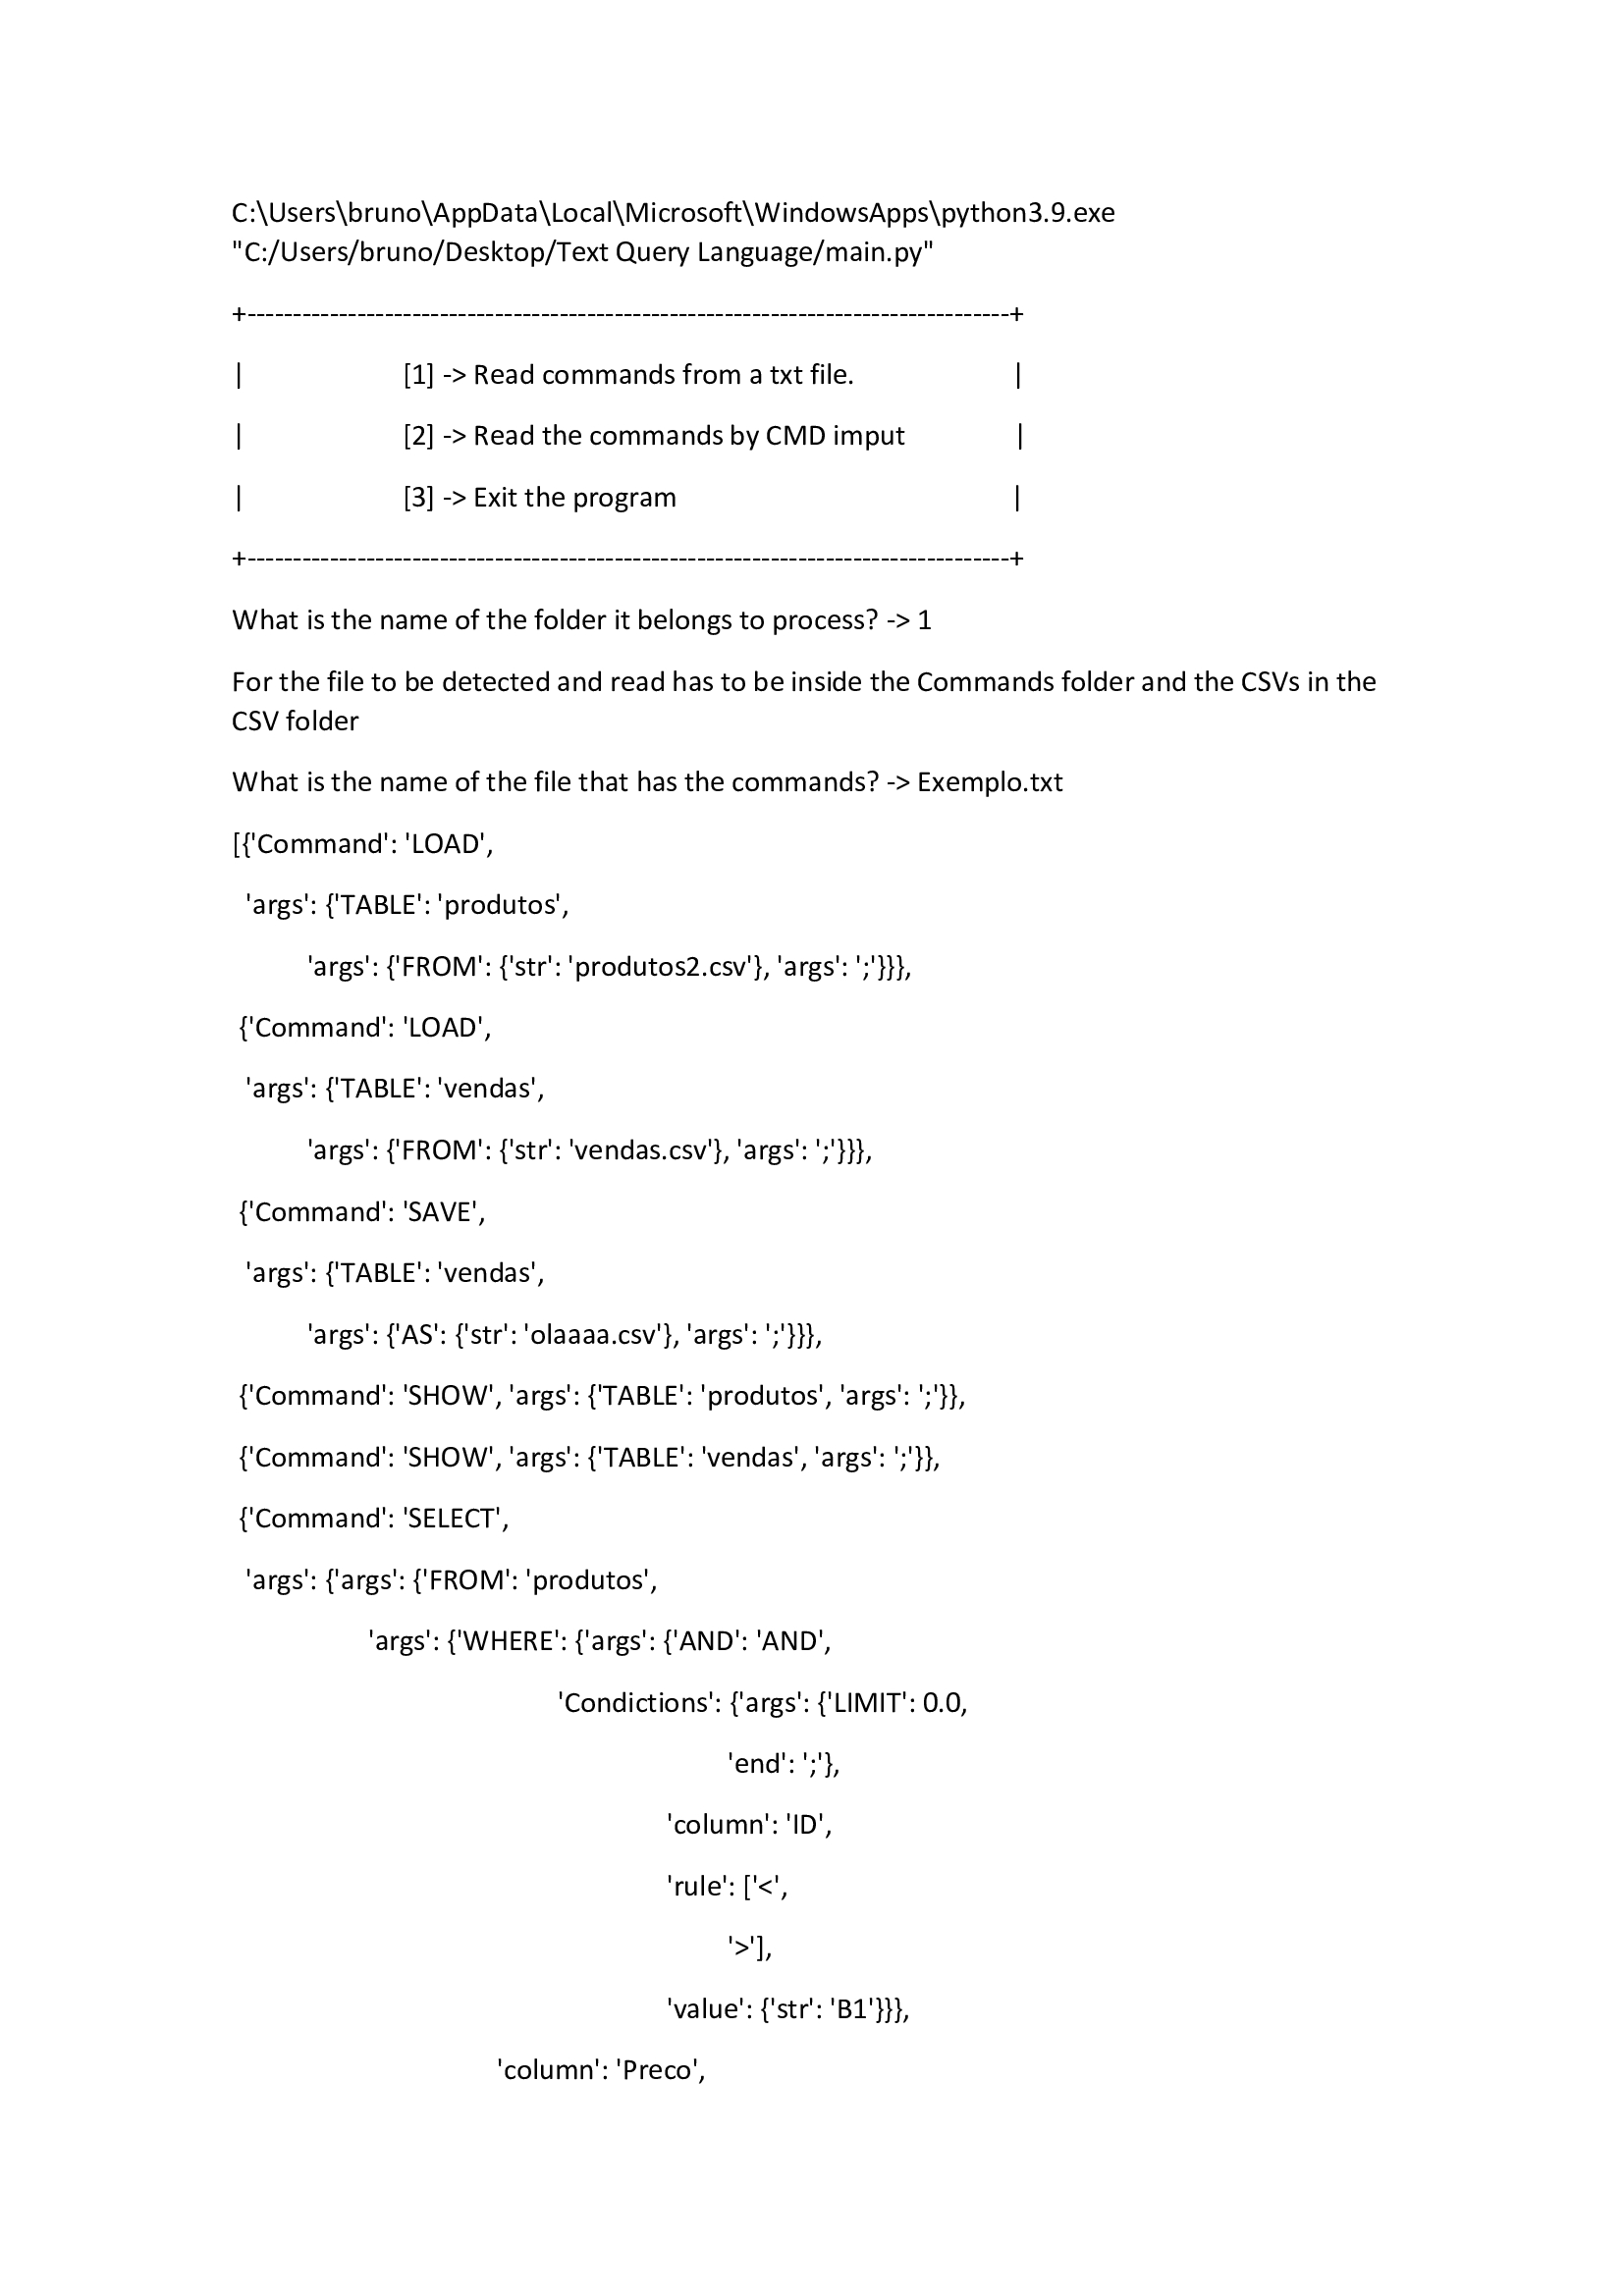
\includegraphics[width=1.3\textwidth]{0}

\noindent
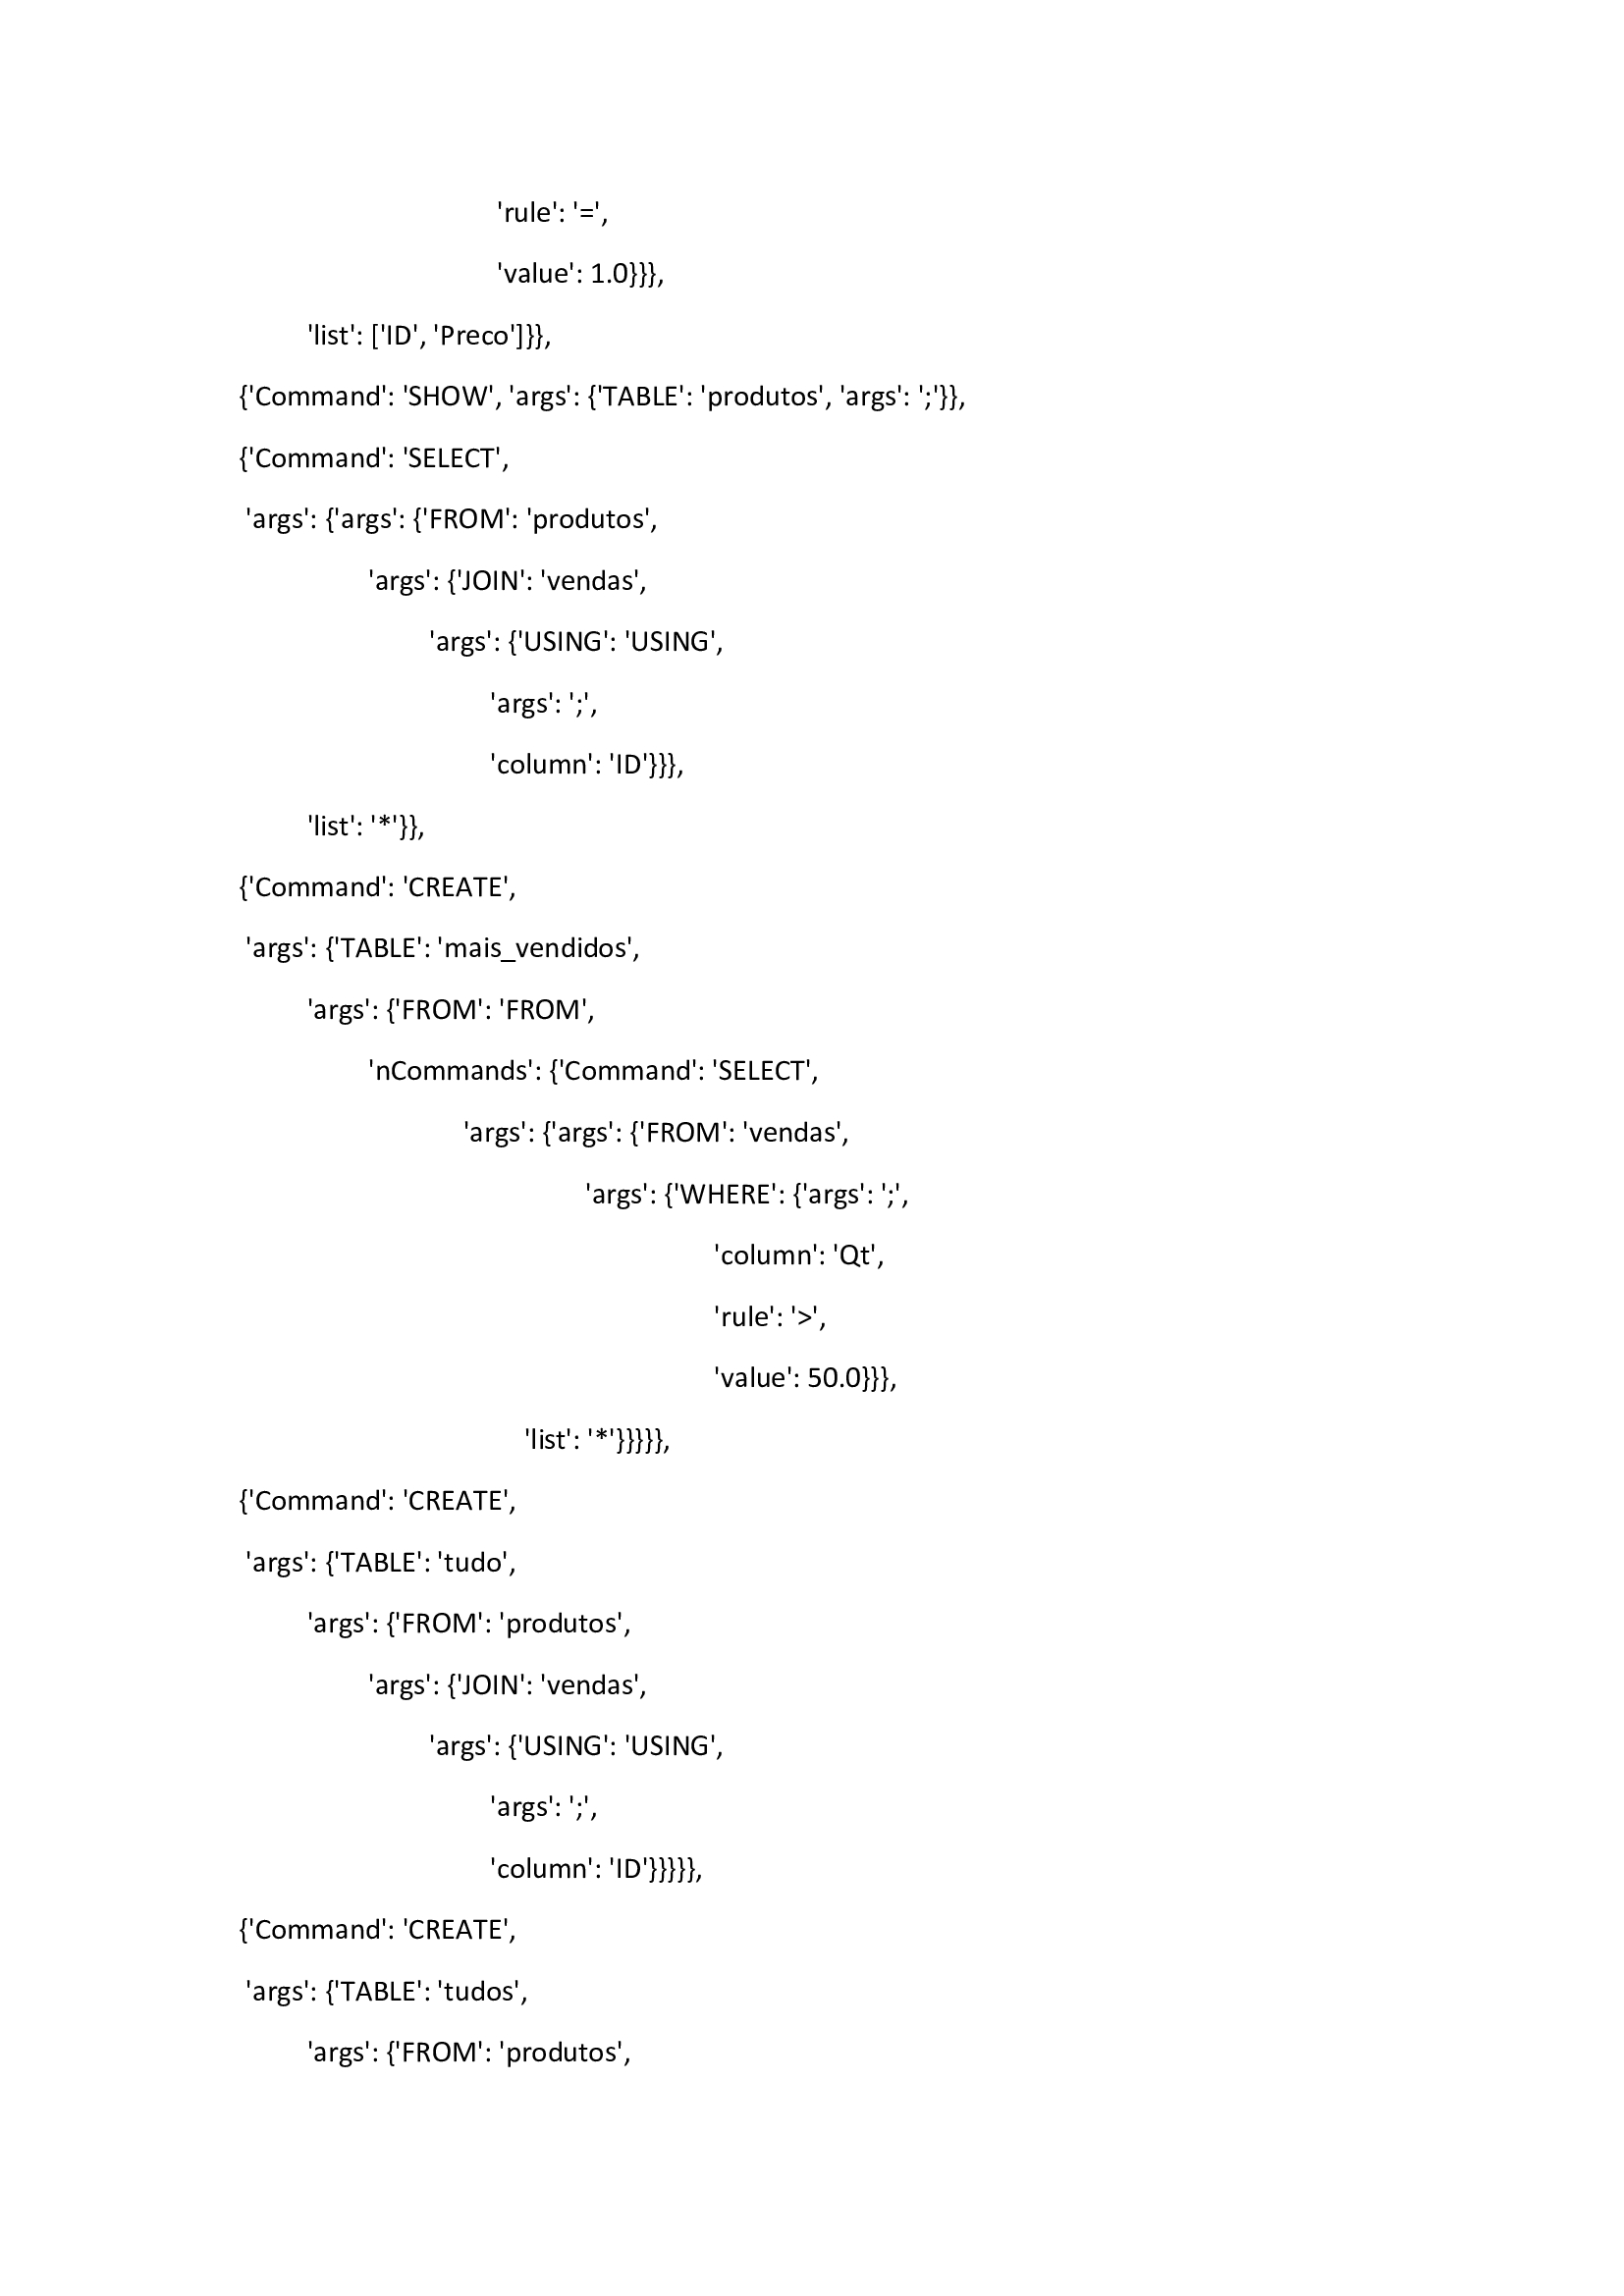
\includegraphics[width=1.3\textwidth]{1}

\noindent
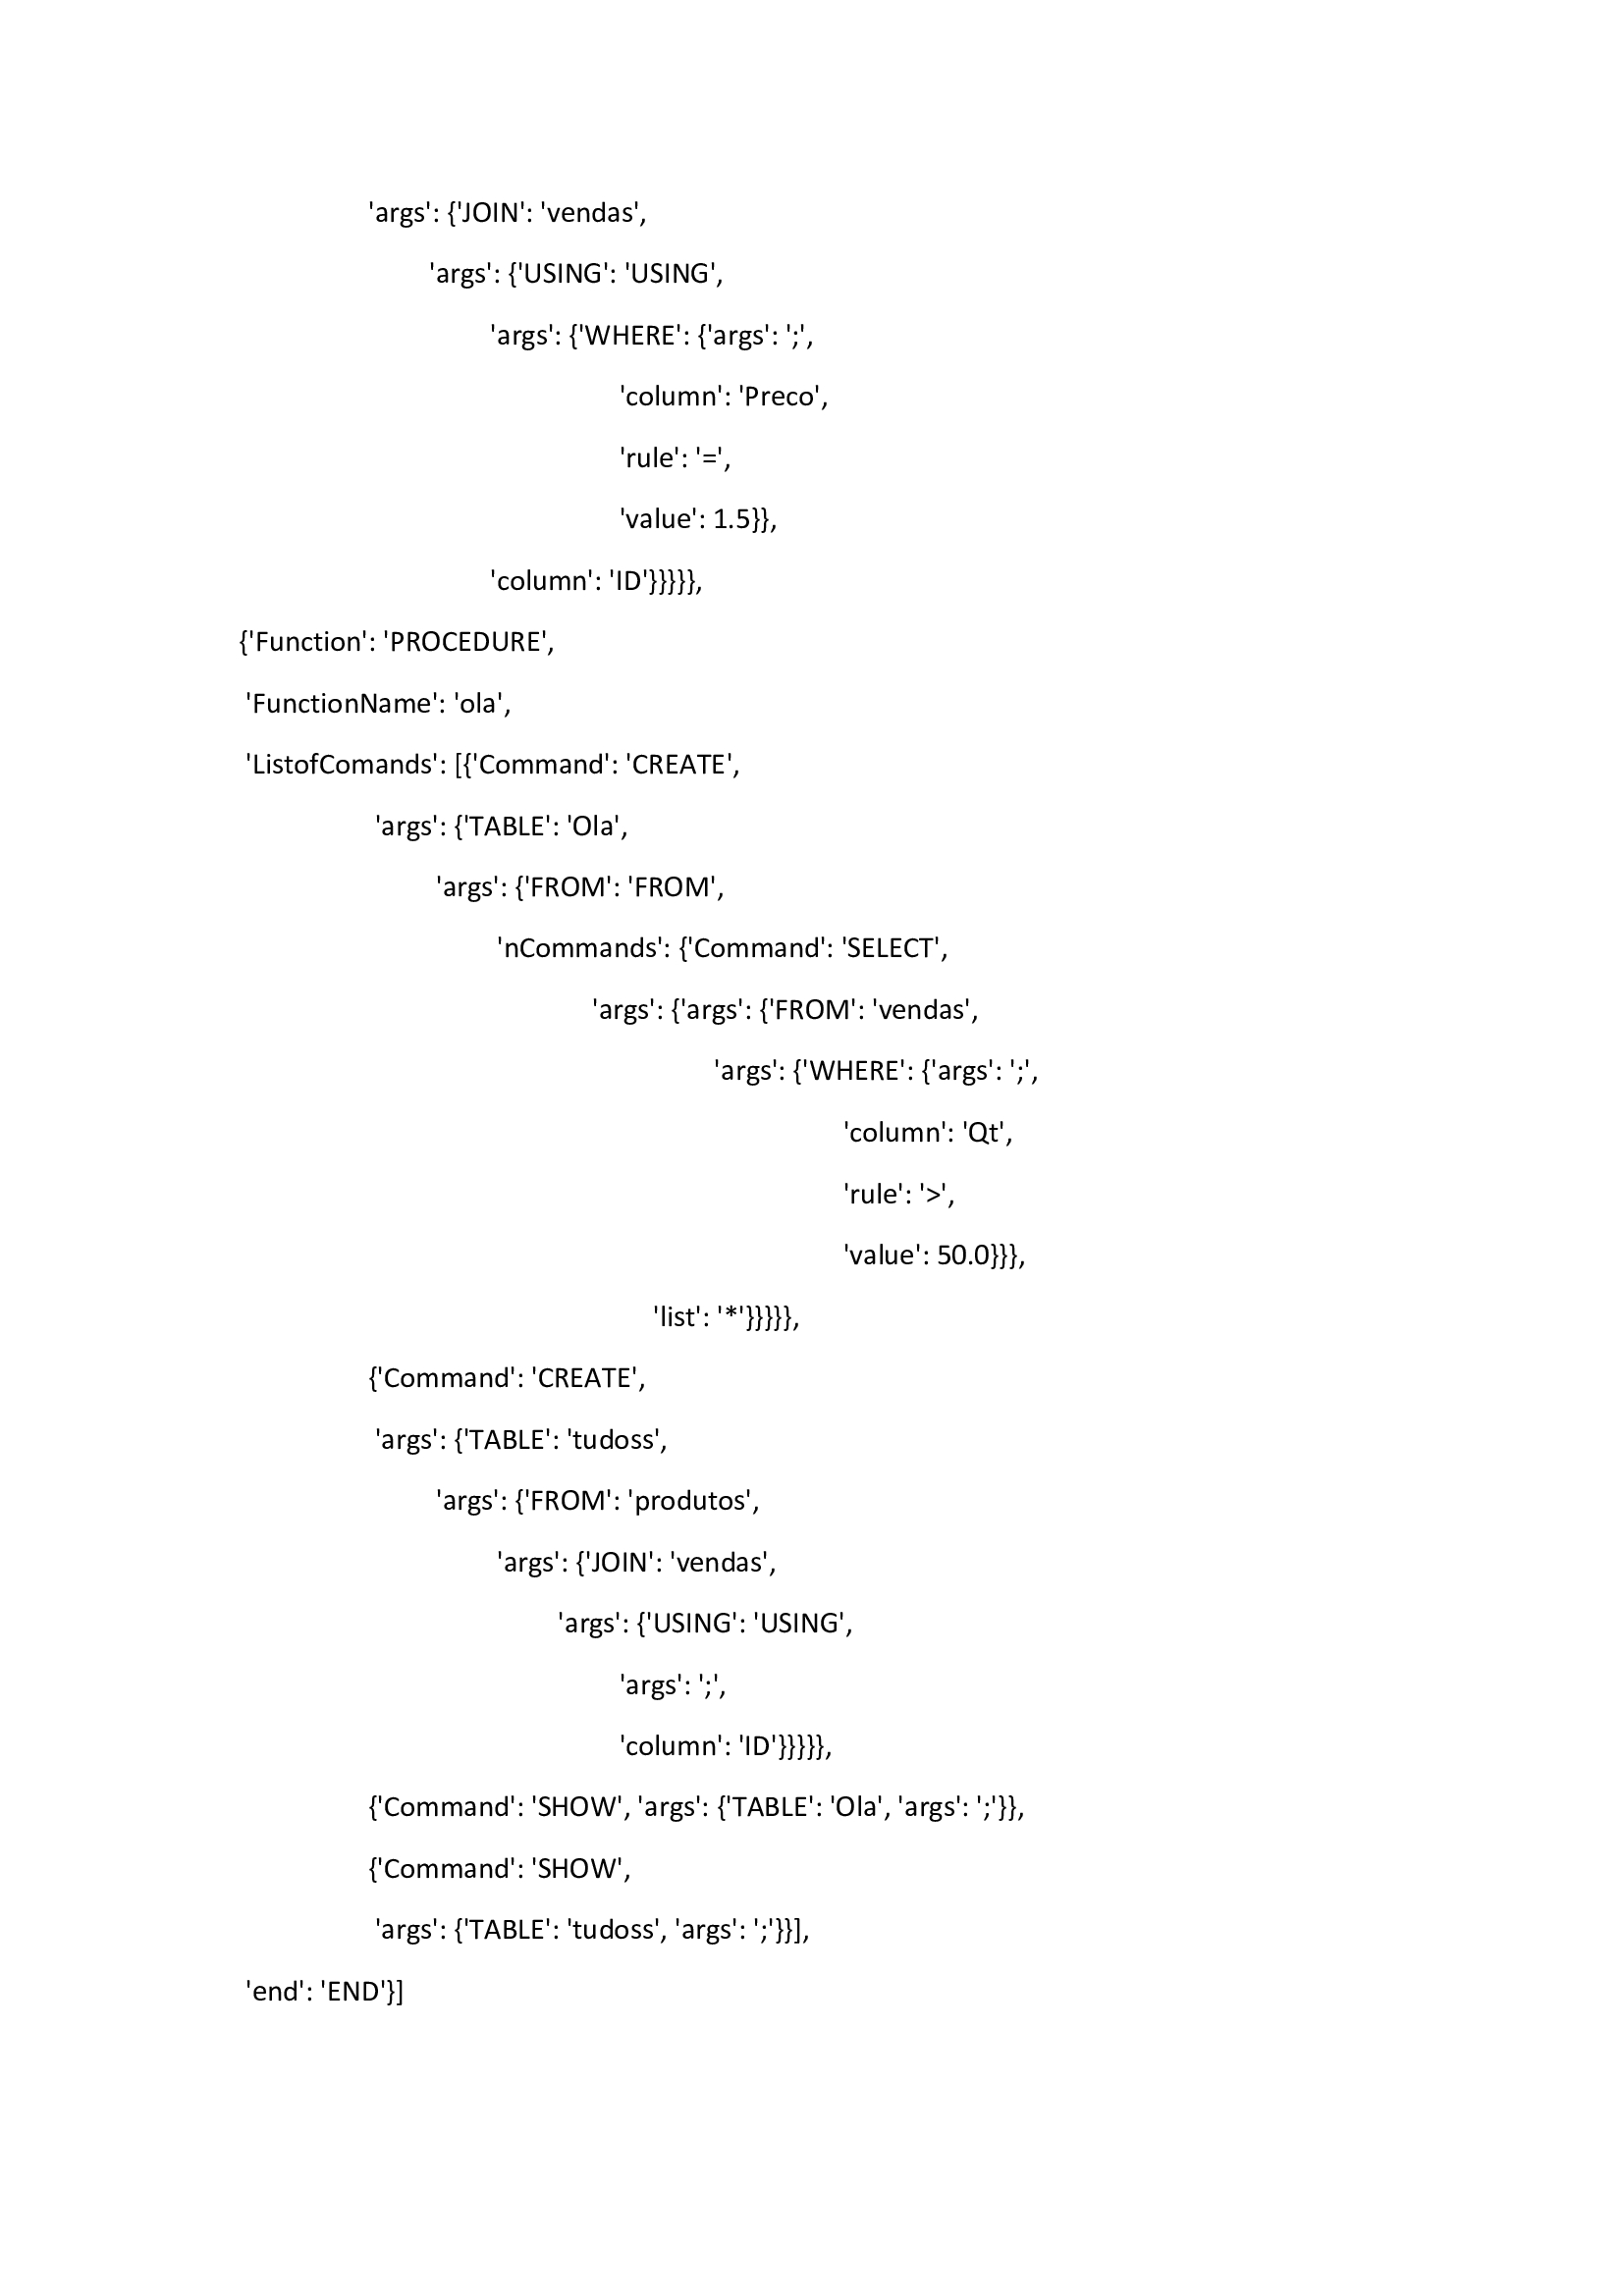
\includegraphics[width=1.3\textwidth]{2}

\noindent
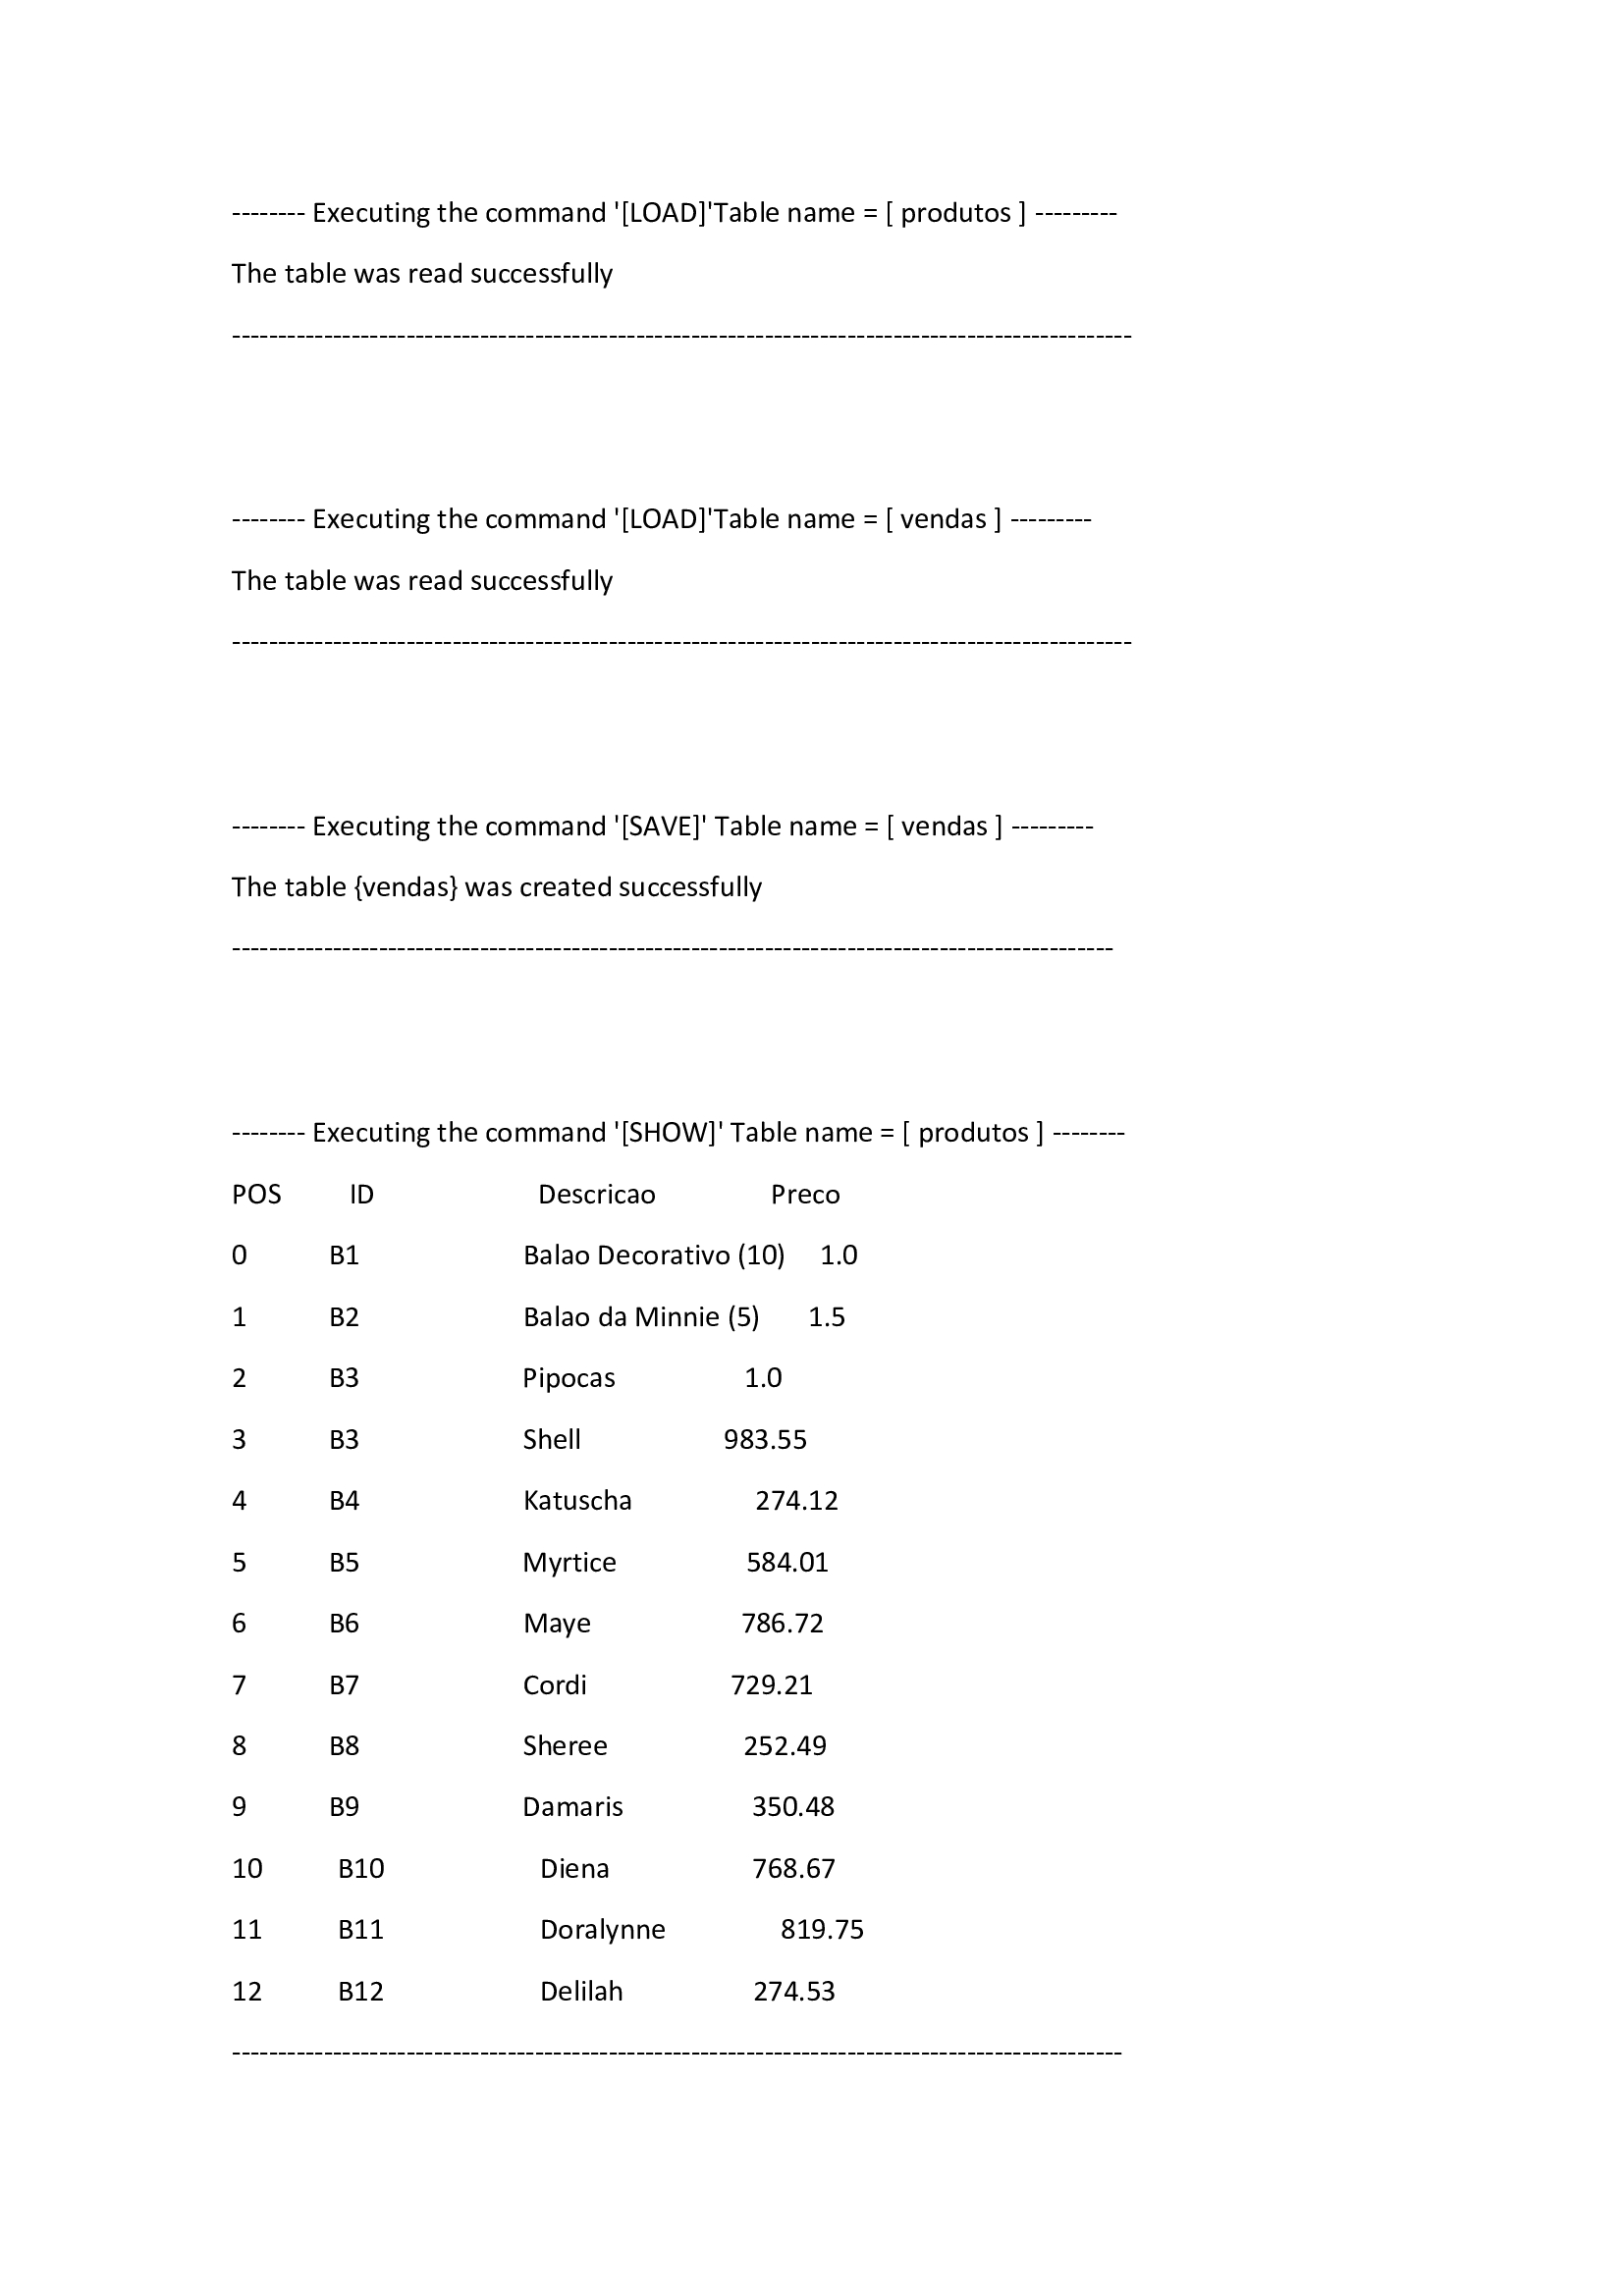
\includegraphics[width=1.3\textwidth]{3}

\noindent
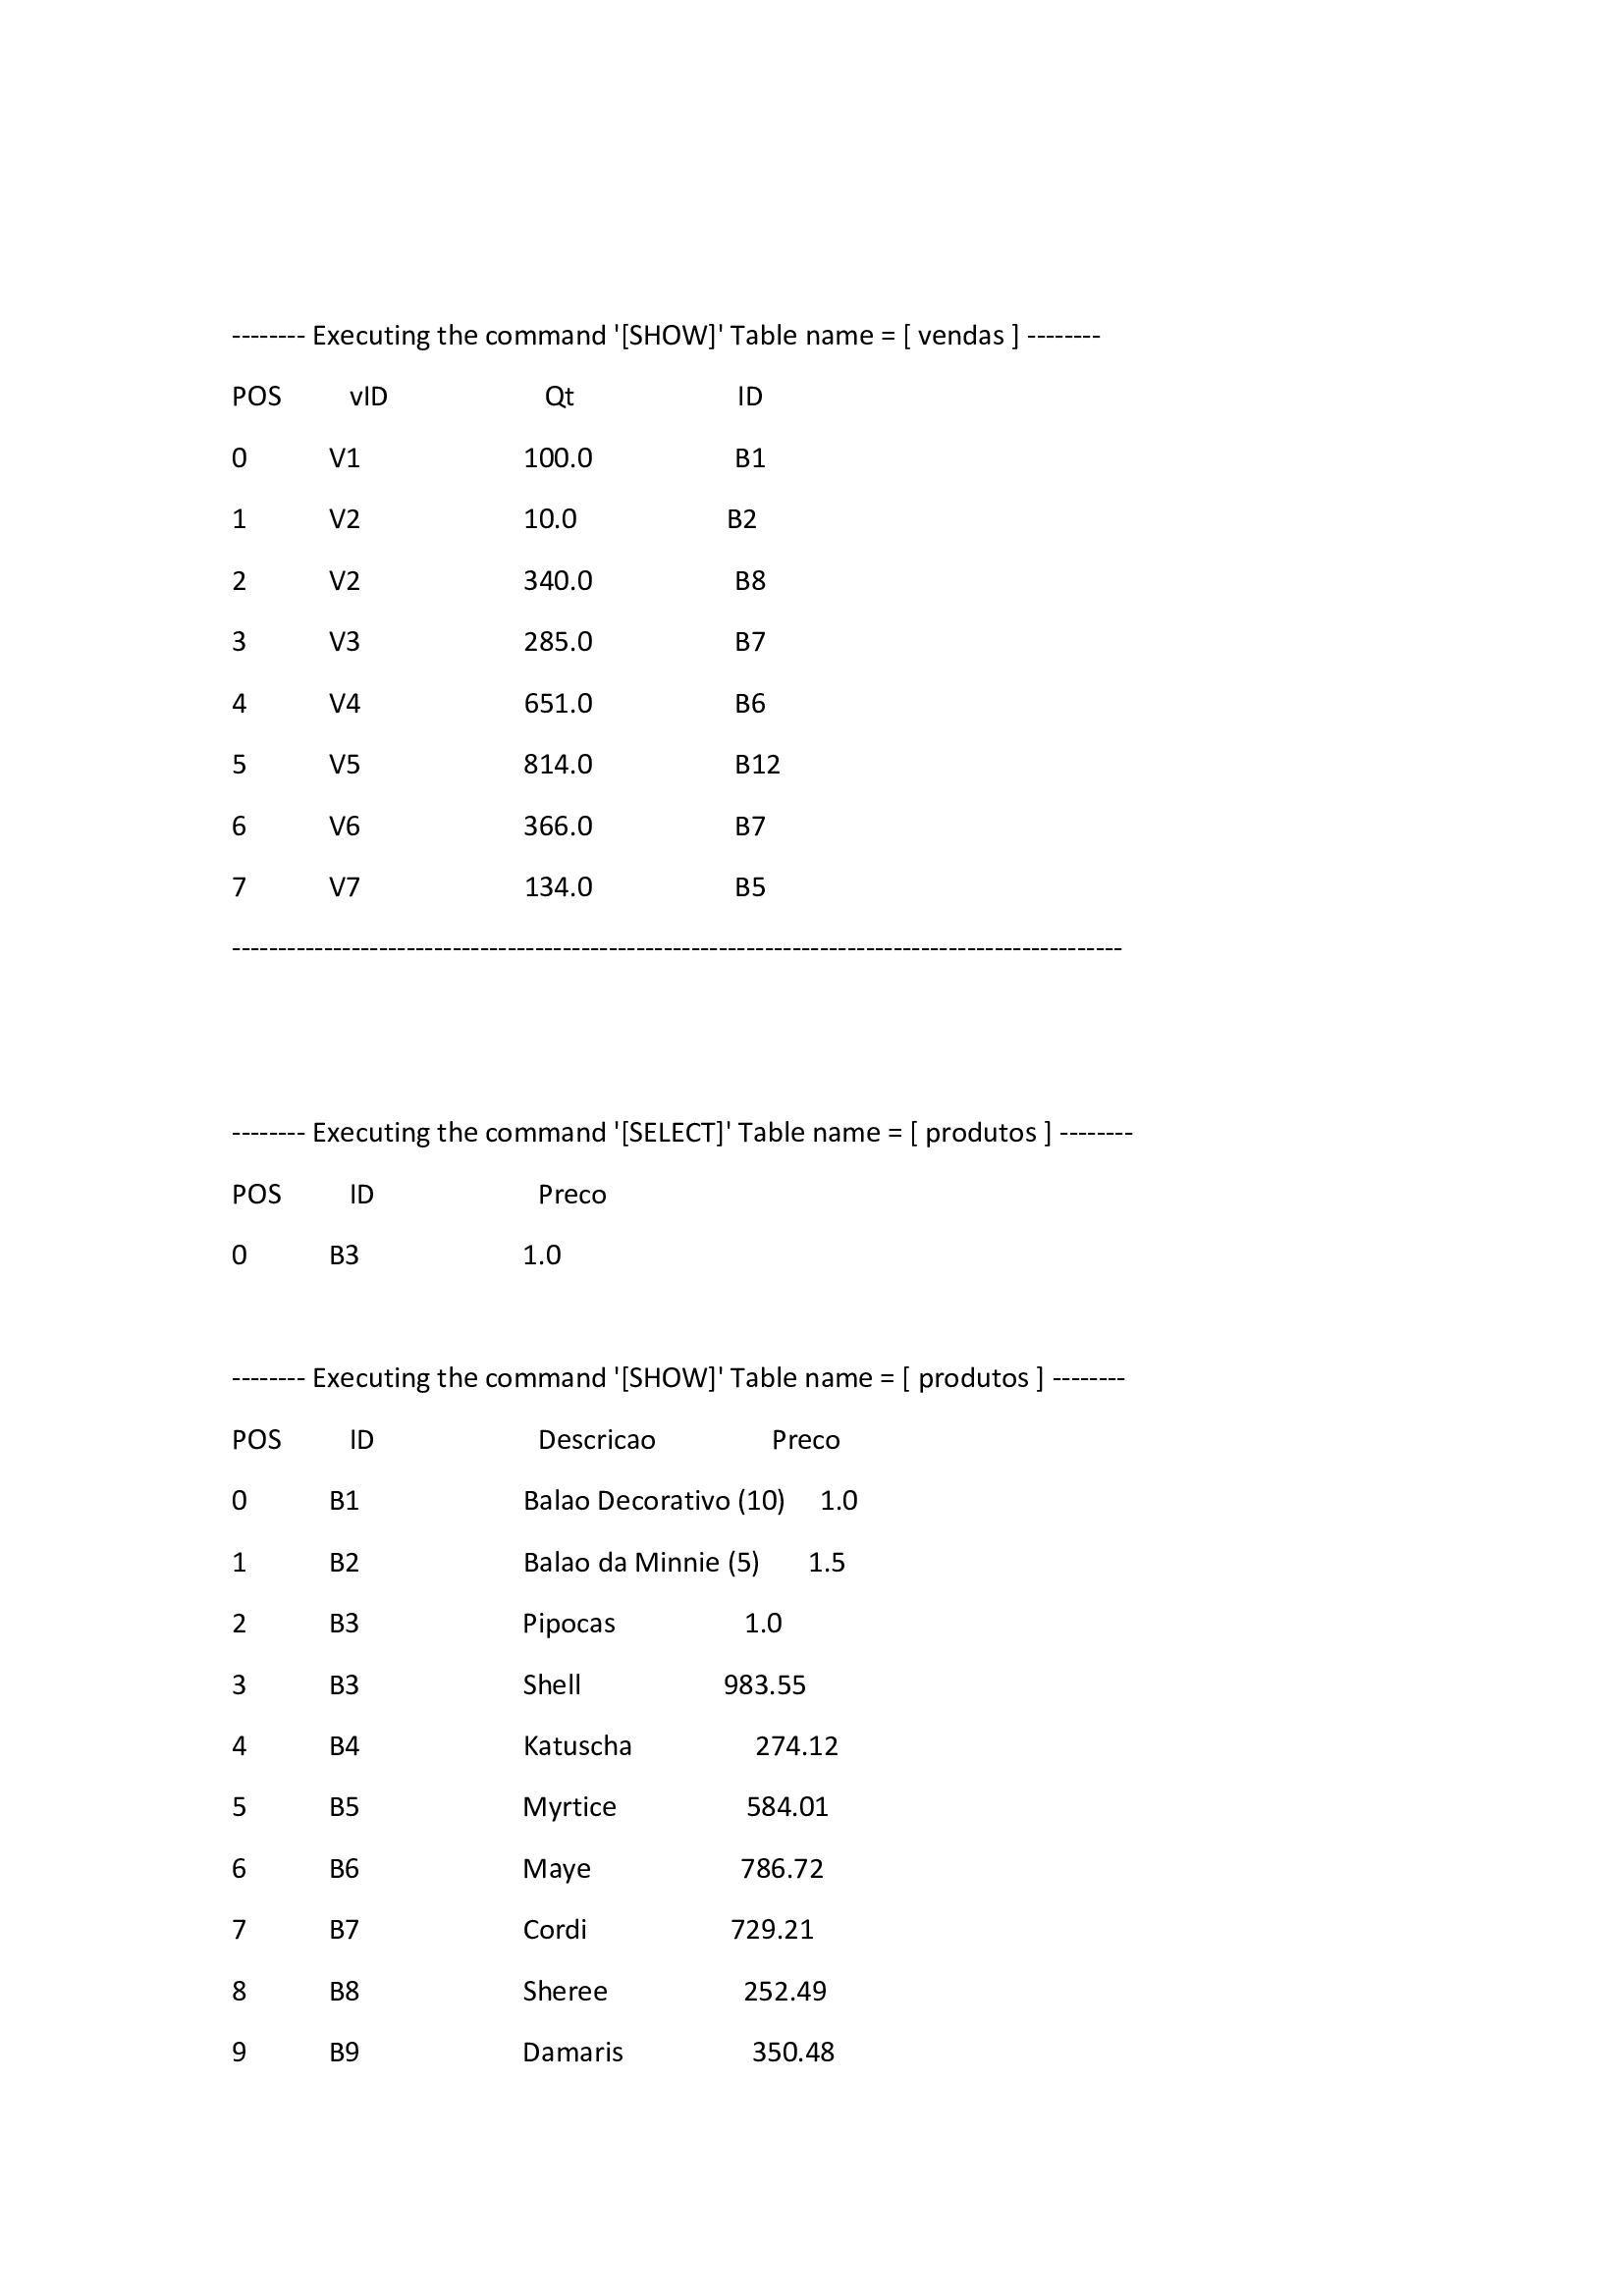
\includegraphics[width=1.3\textwidth]{4}

\noindent
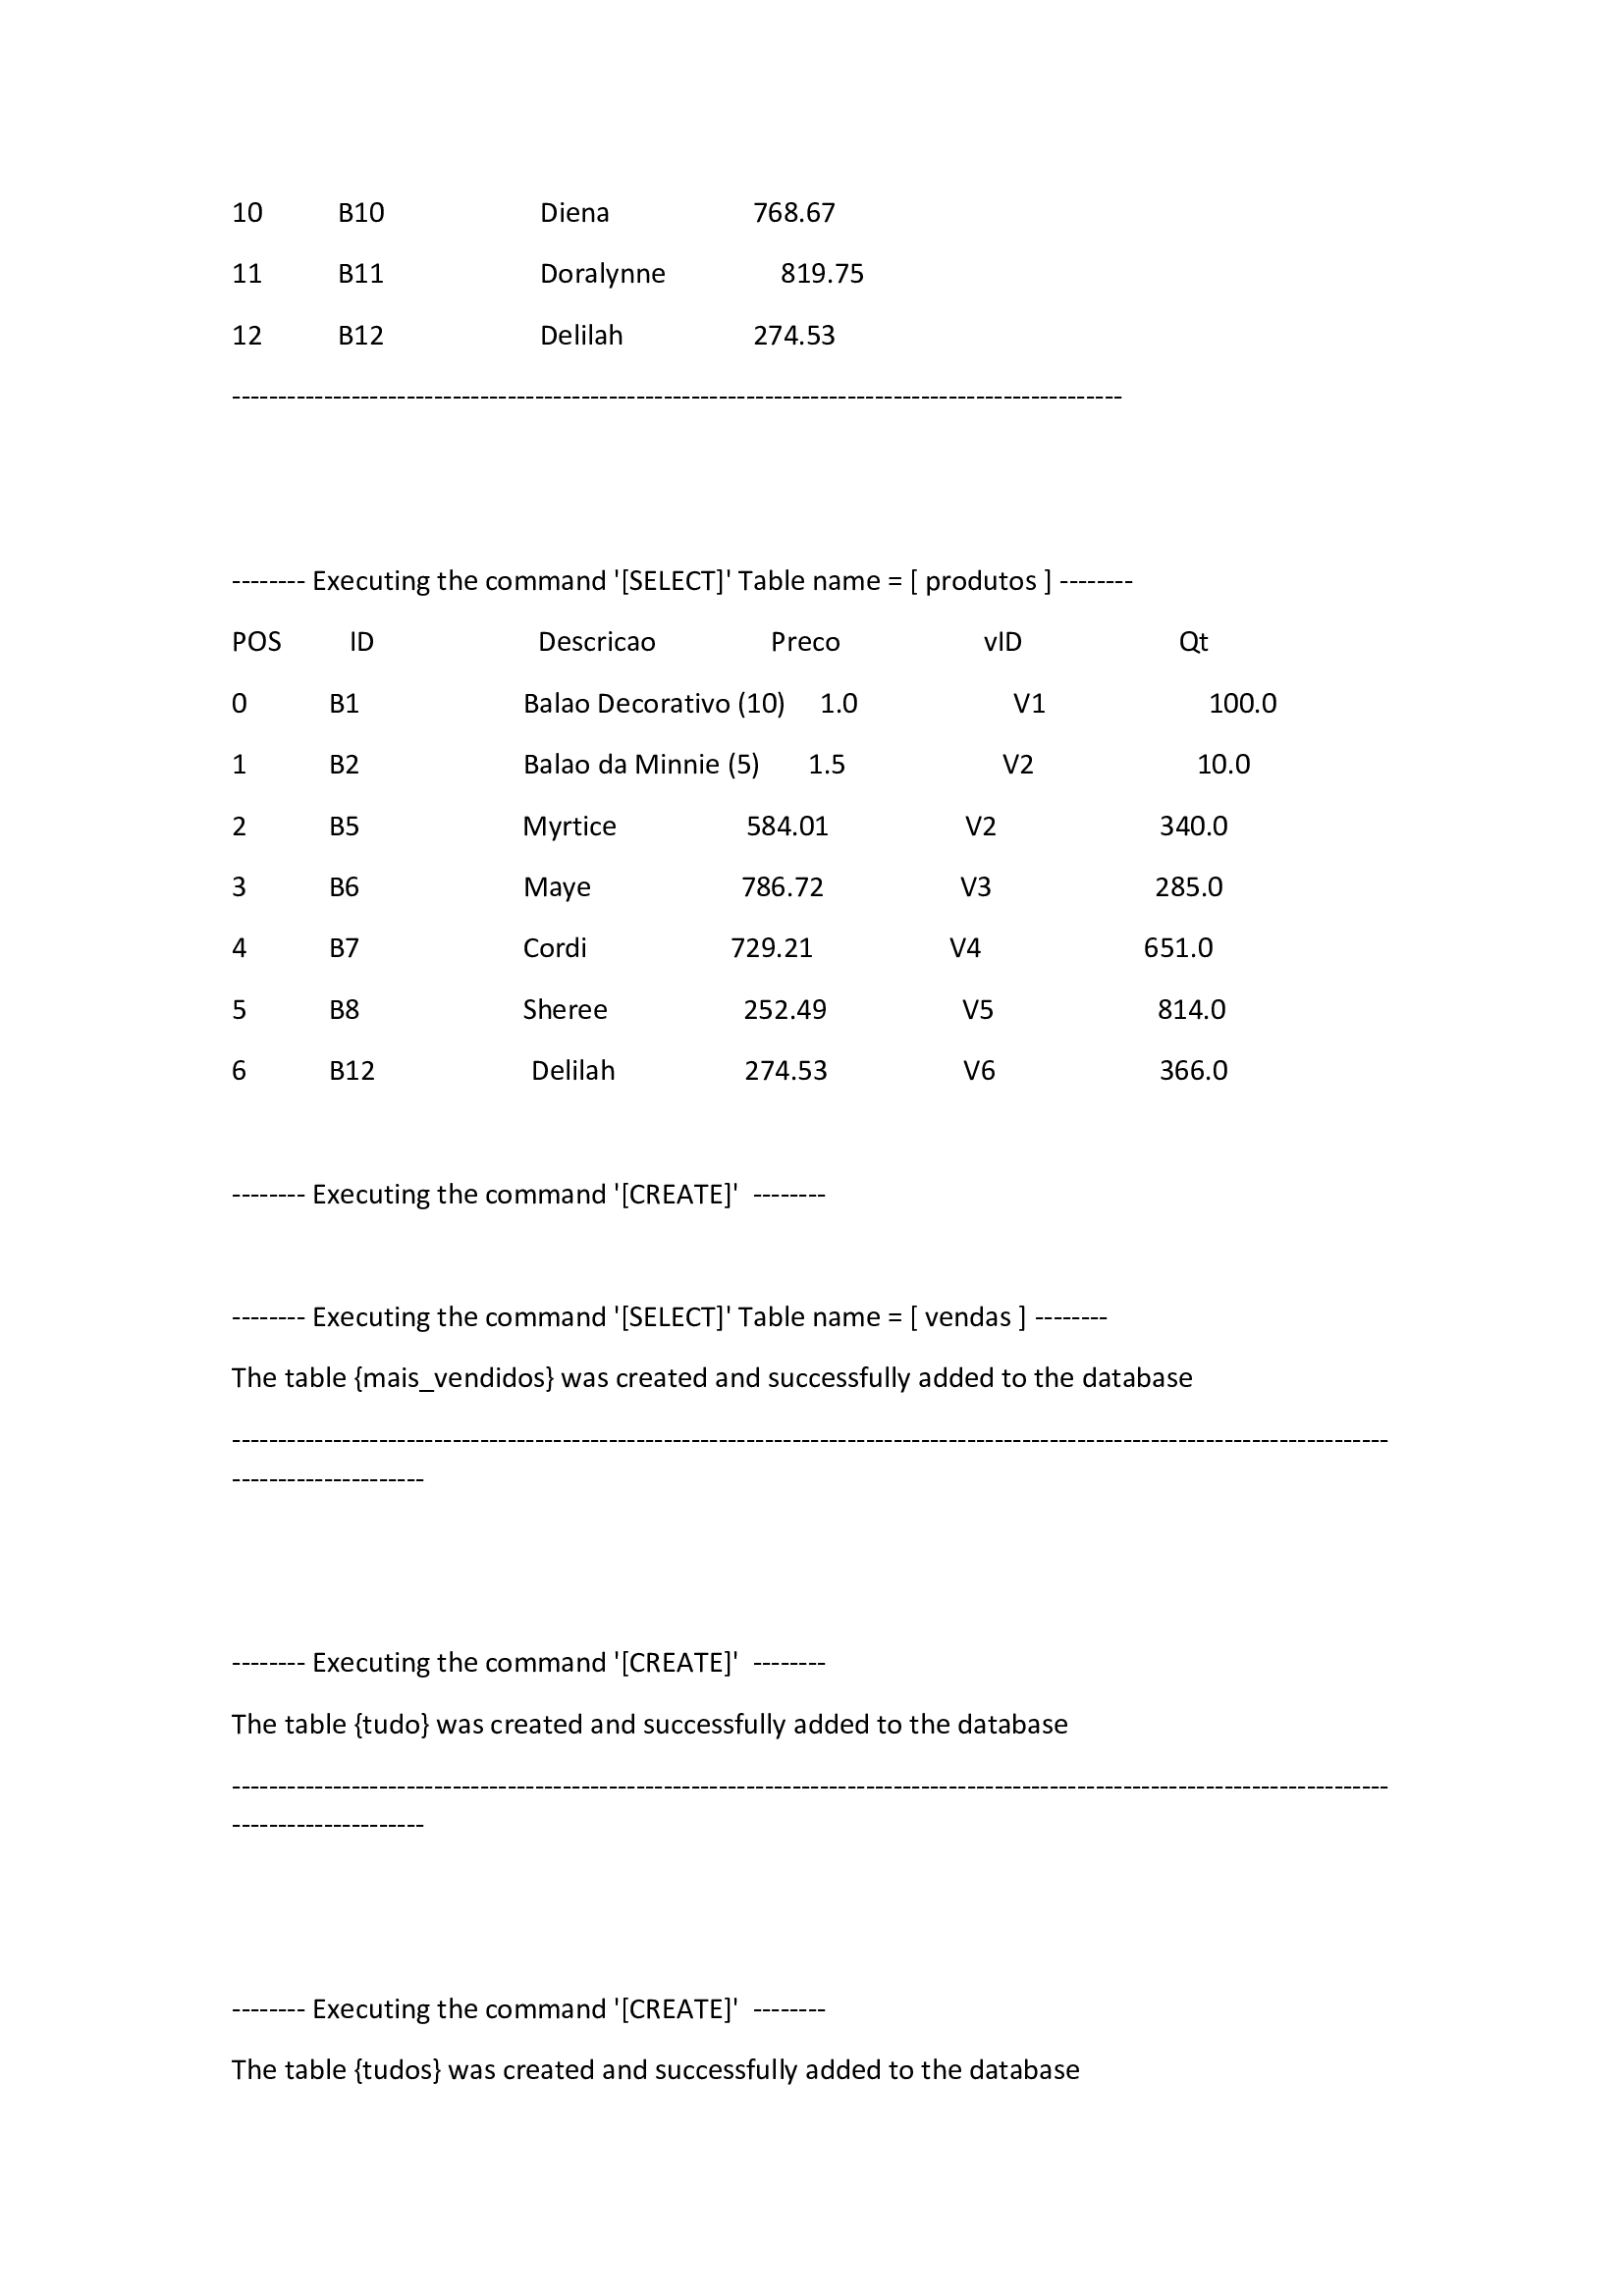
\includegraphics[width=1.3\textwidth]{5}

\noindent
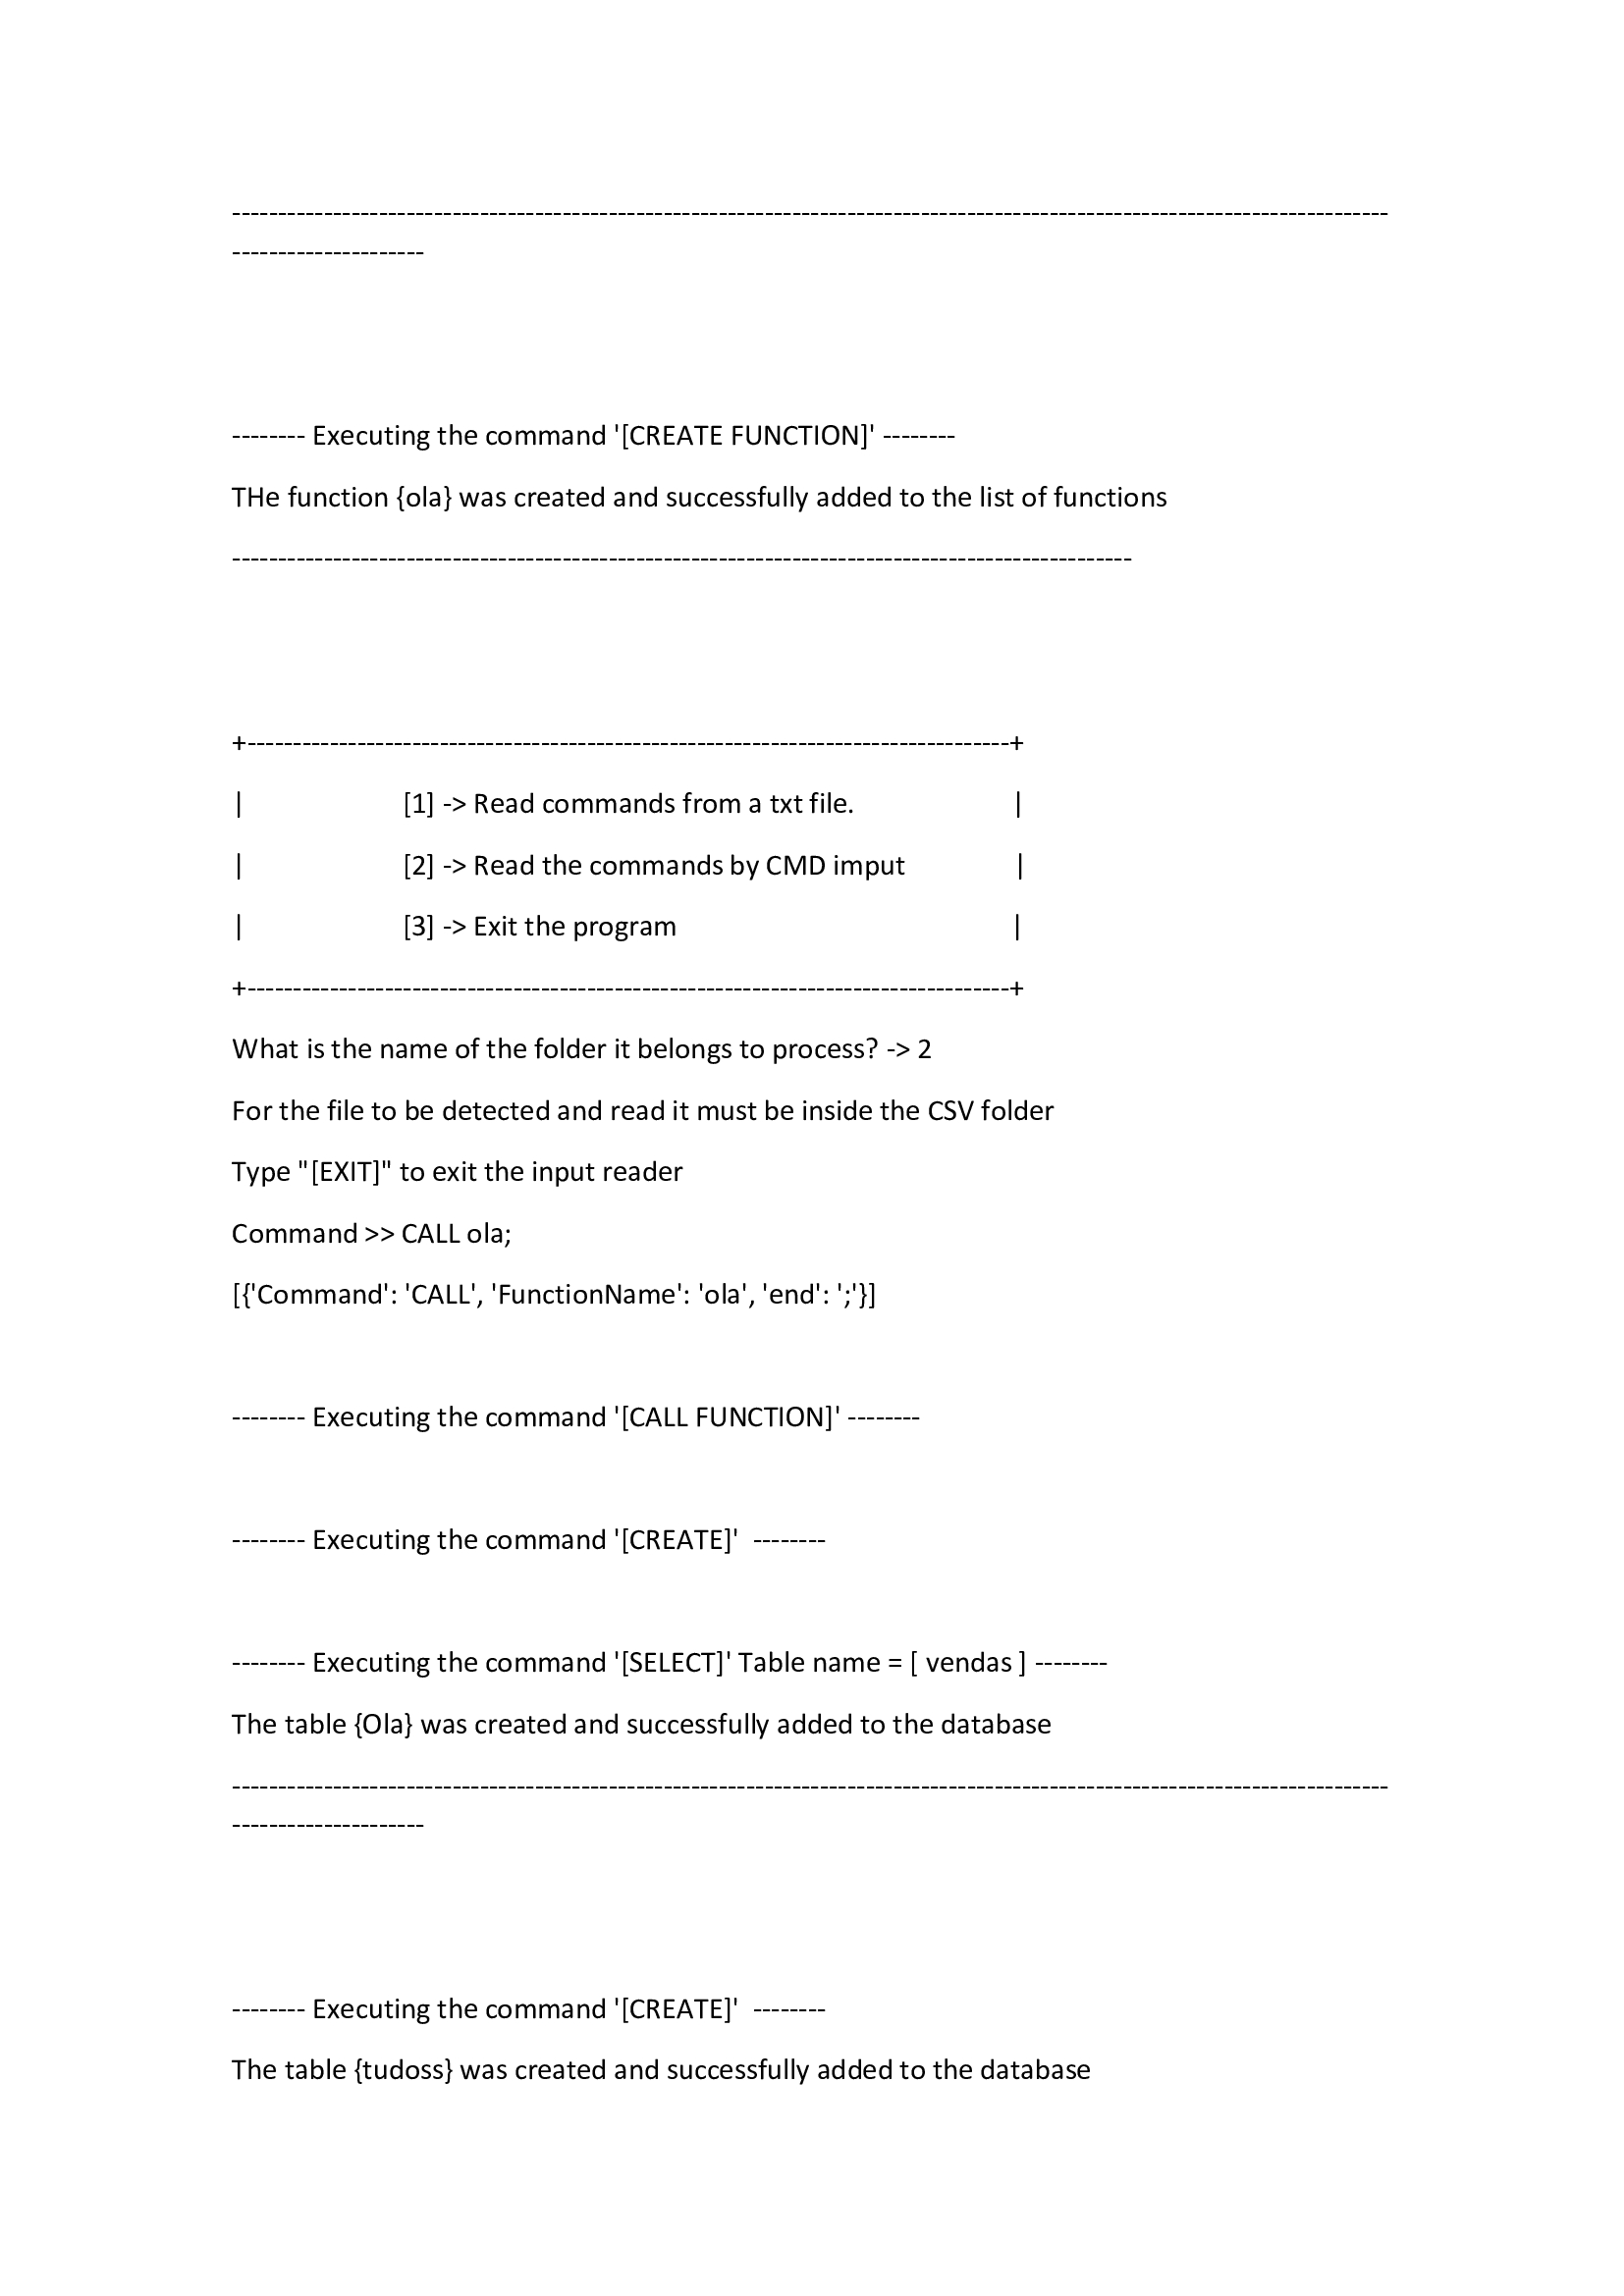
\includegraphics[width=1.3\textwidth]{6}

\noindent
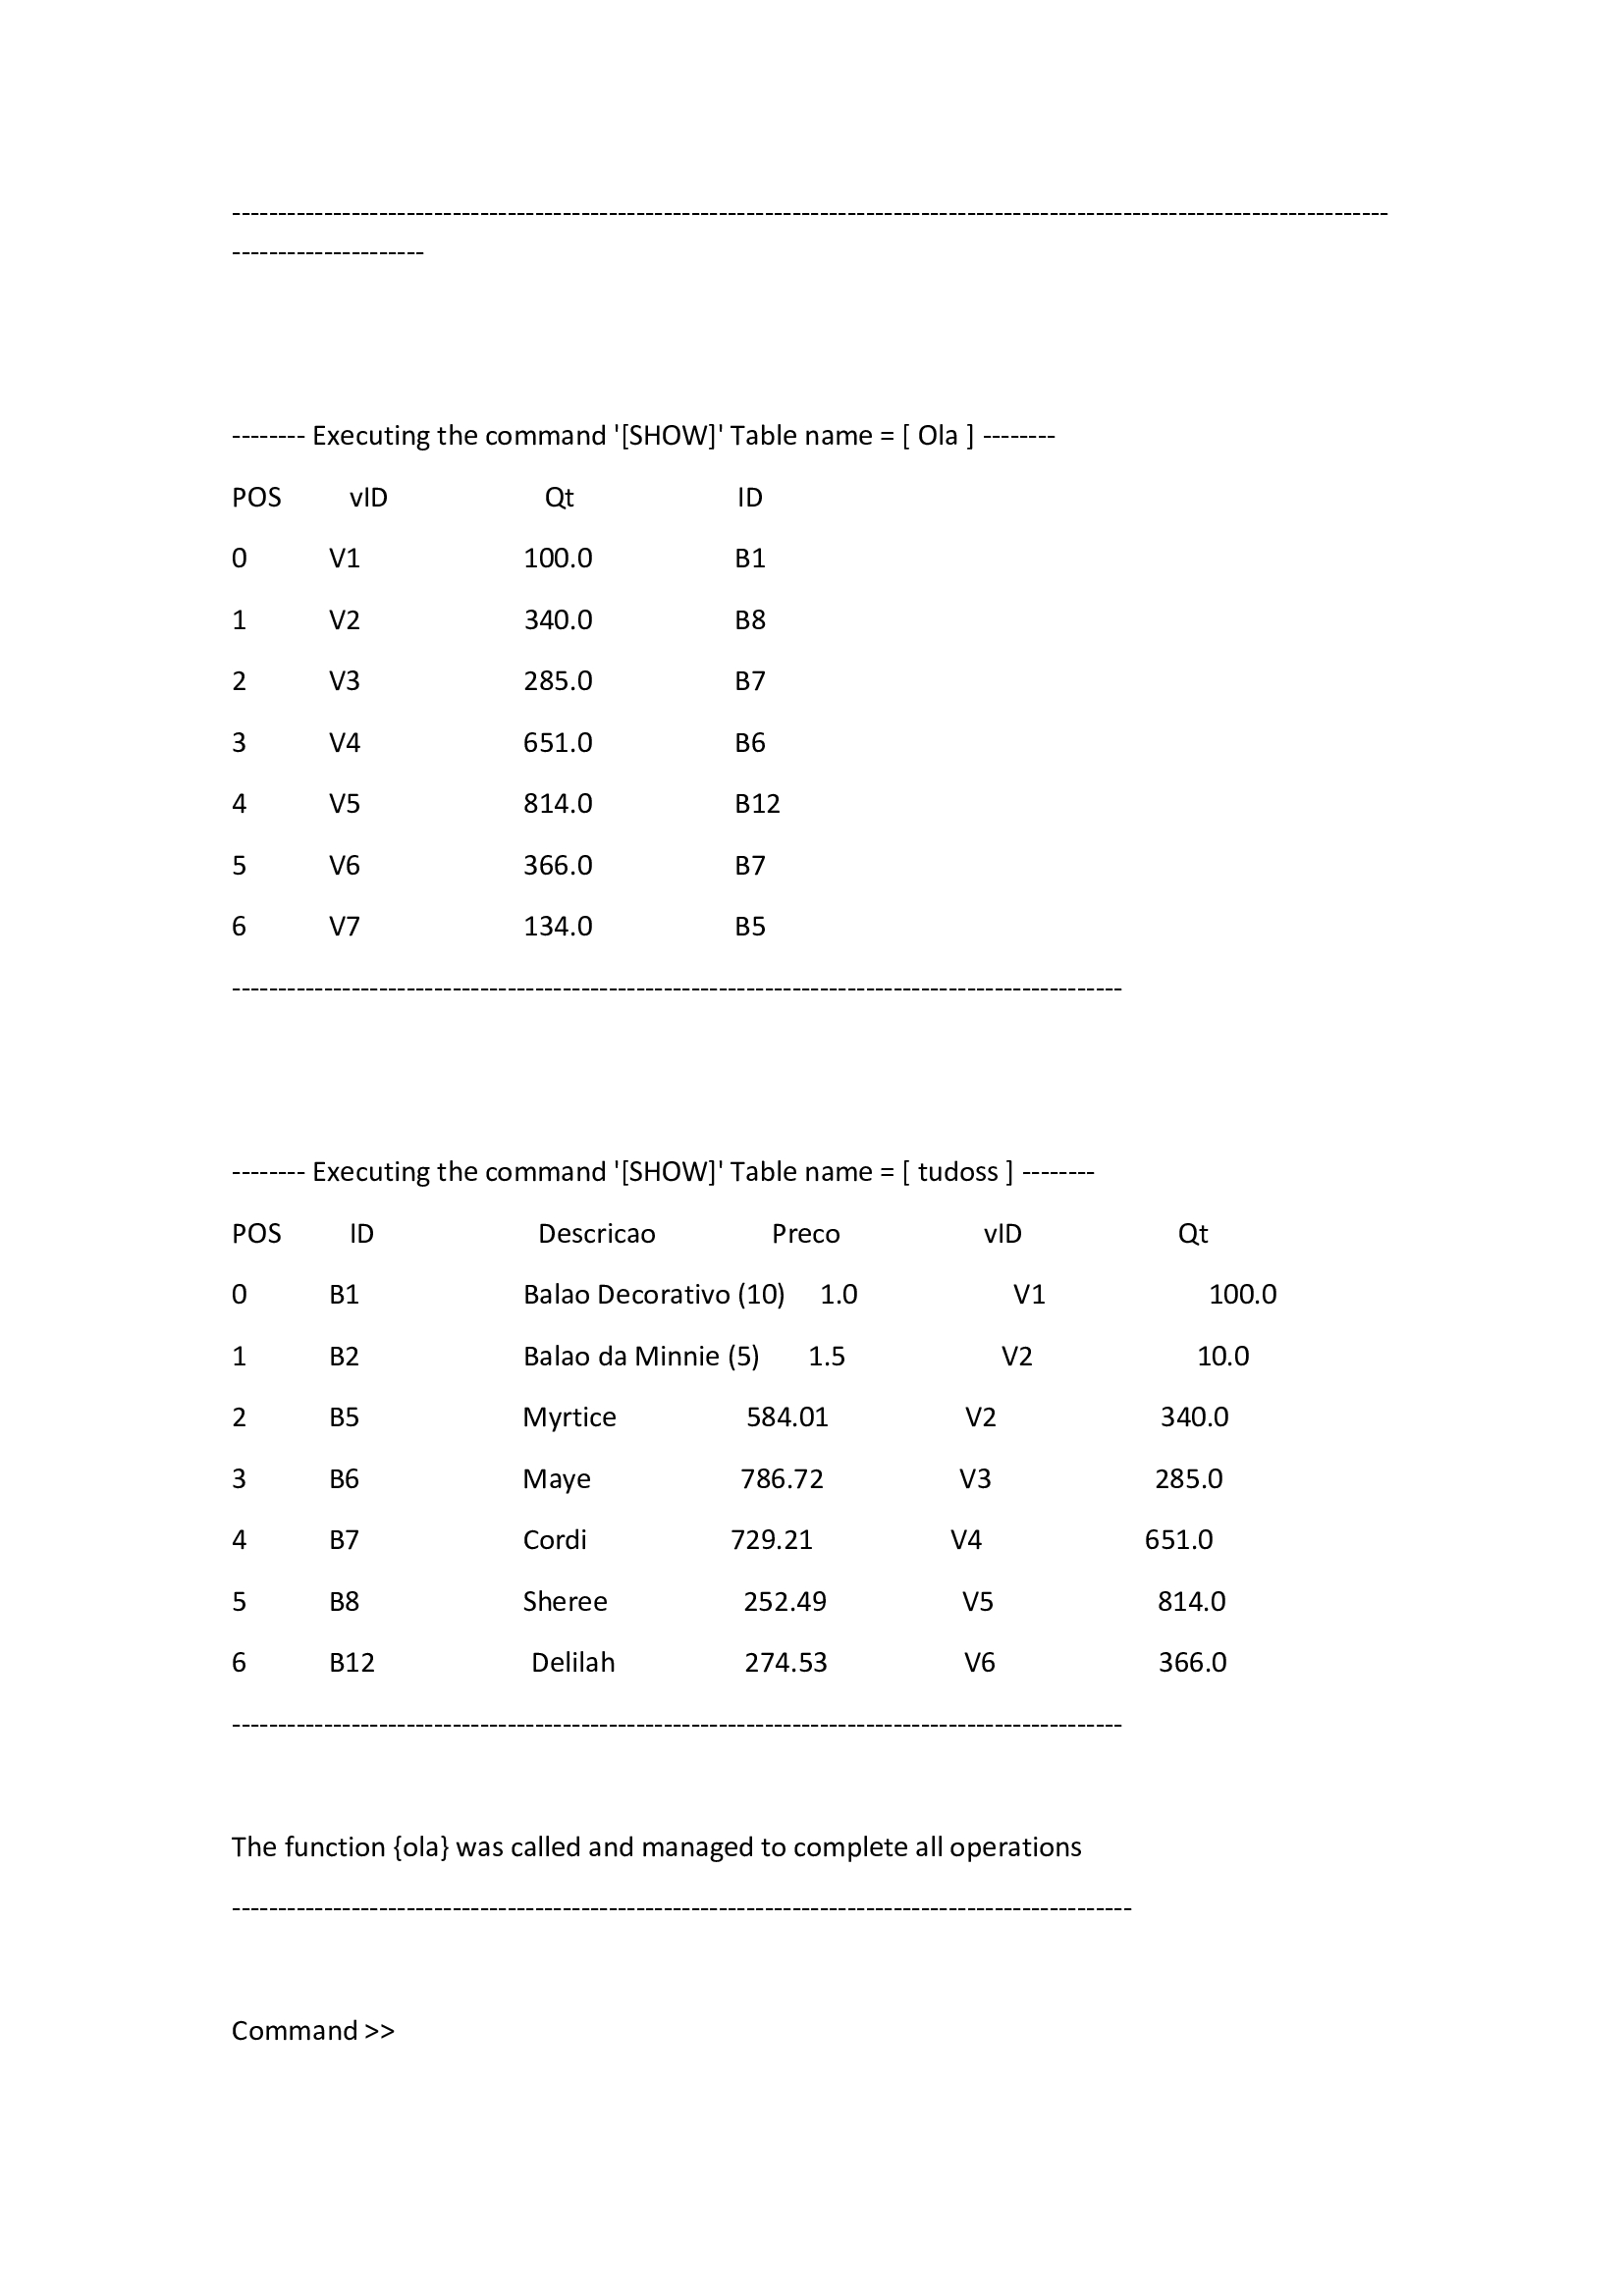
\includegraphics[width=1.3\textwidth]{7}




\end{document}